\section{Implementation of Model Fragmentation}
\label{sec:implemention}

In previous sections, we introduced model fragmentation, a specific fragmentation strategy, and the theoretical merits of fragmentation. In this section, we present a framework that realizes model fragmentation and implements the meta-model based fragmentation strategy. The framework is called \emph{EMFFrag}.

The rational behind EMFFrag is to (re)use EMF resource as much as possible. EMF resource already realize partial model persistence, they manage inter-resource references through proxies, they lazy-load, can be added and removed, objects can be moved between resources, etc. EMFFrag only uses and specialized the existing implementations of EMF resources.

\begin{figure}
  \centering
  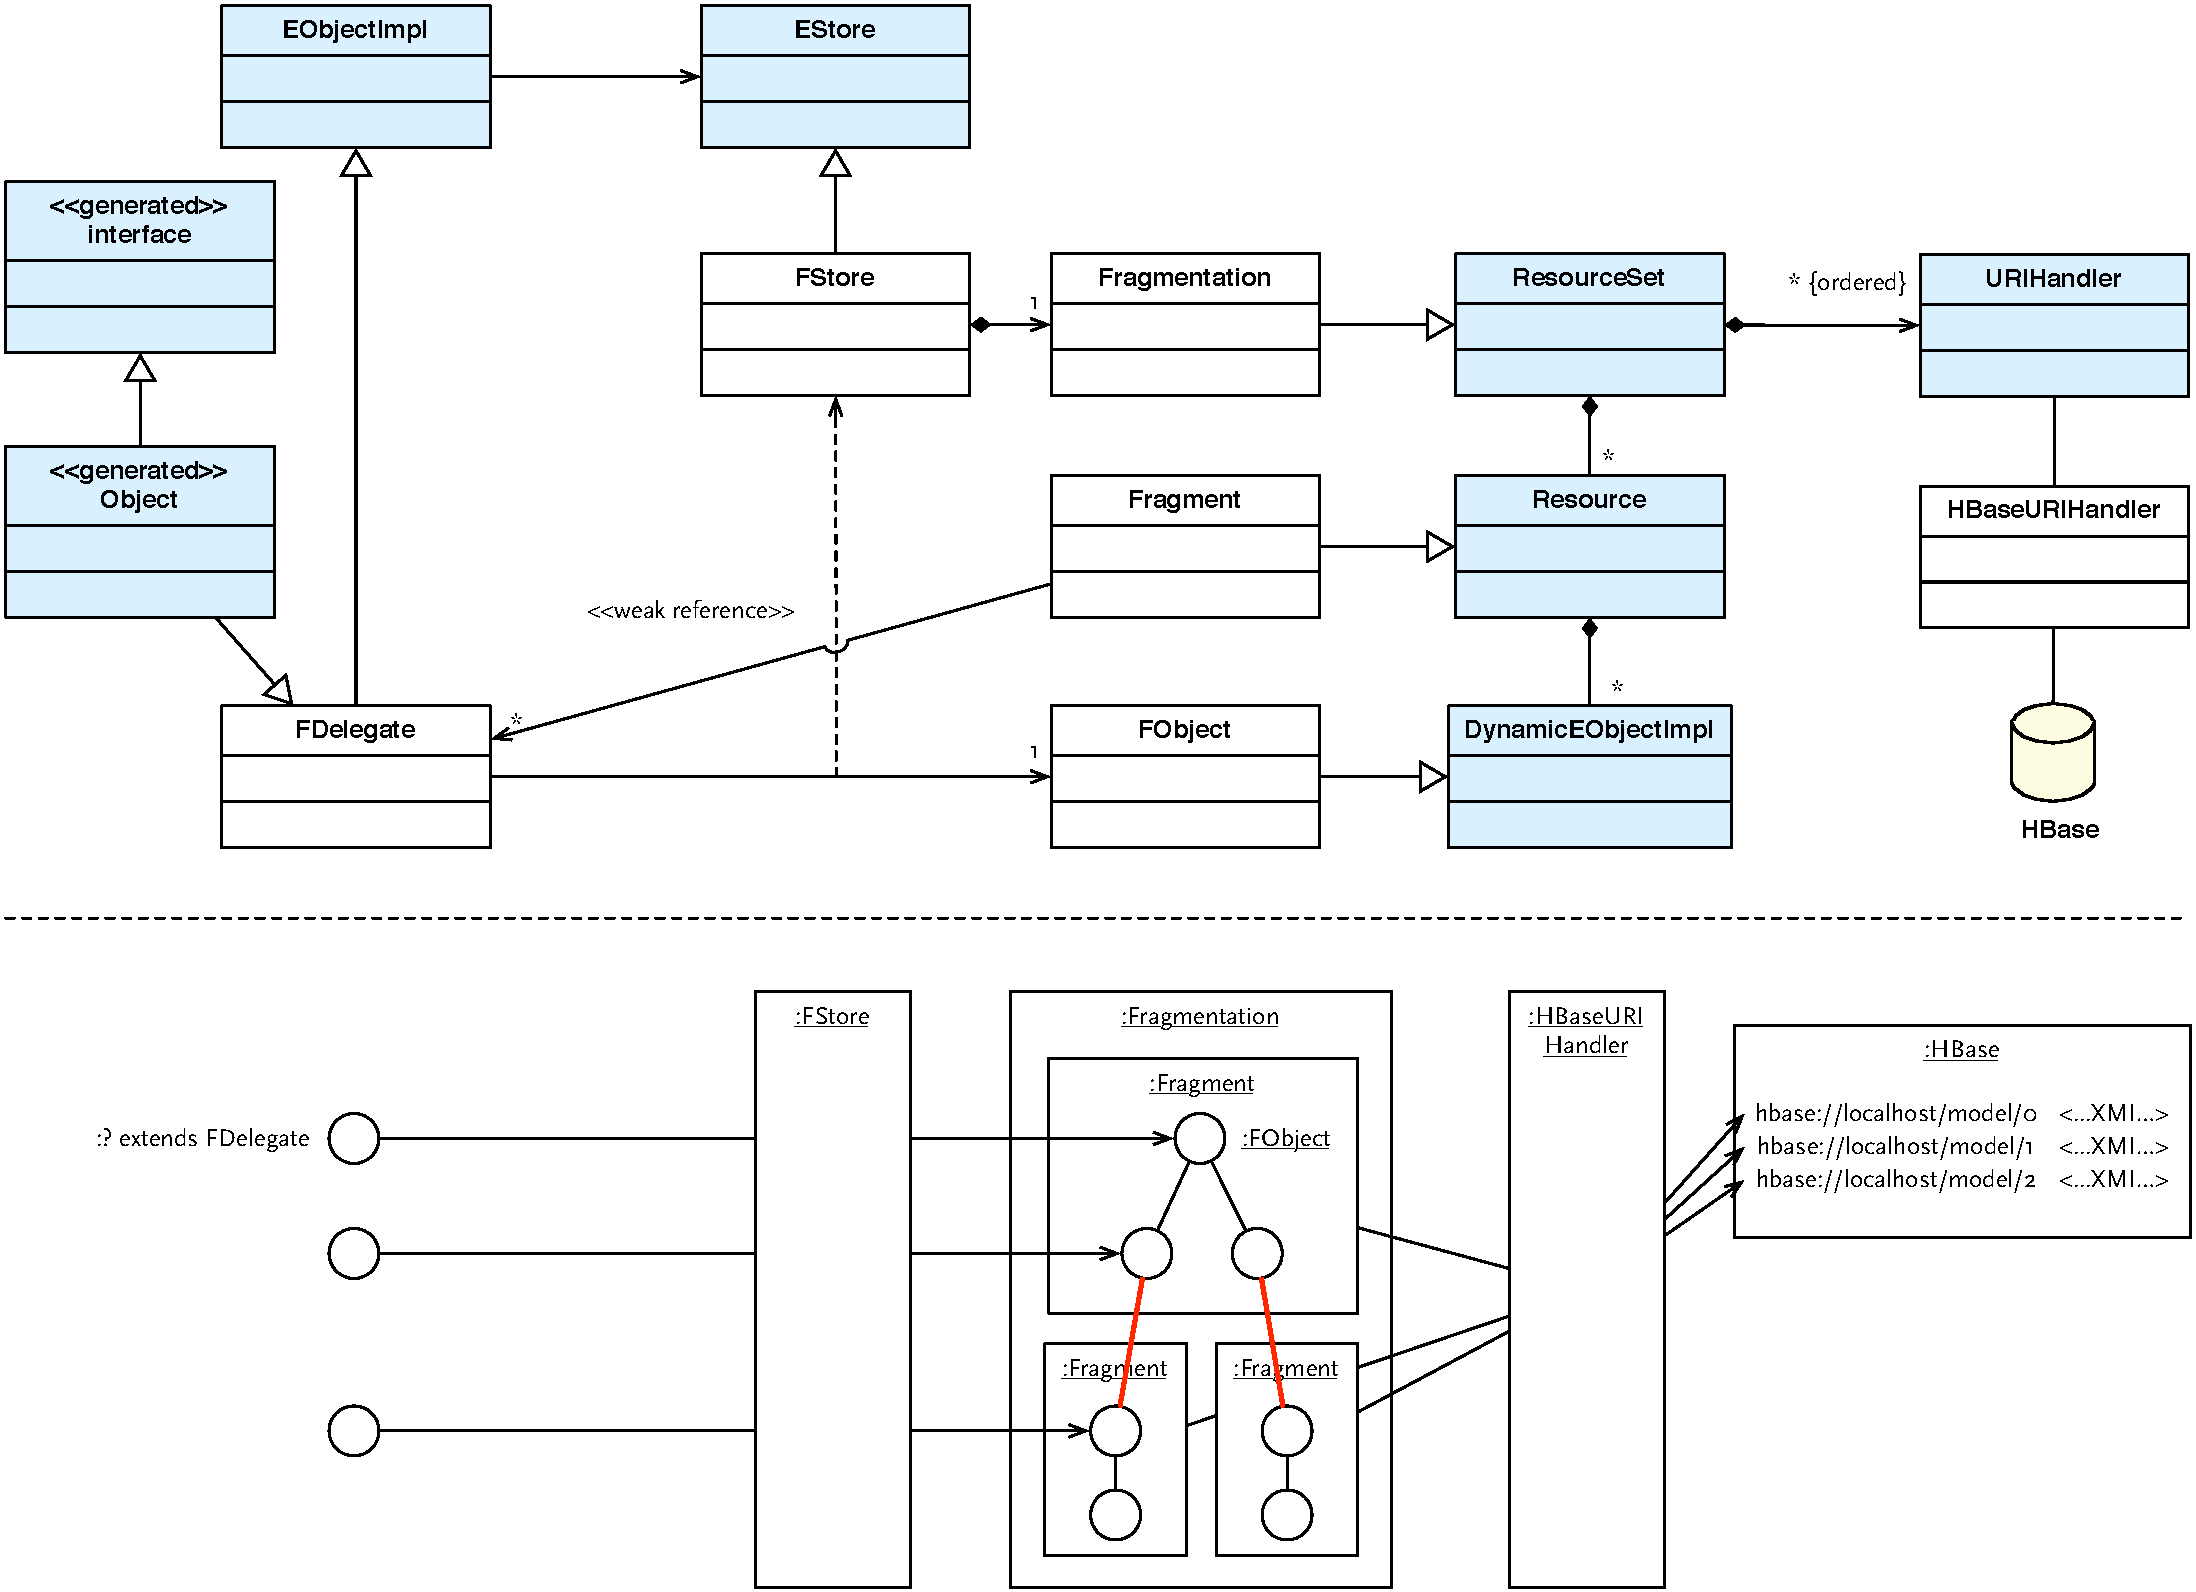
\includegraphics[width=\linewidth]{figures/architecture}
  \caption{EMFFrag architecture and example fragmentation.}
  \label{fig:architecture}
\end{figure}

Fig.~\ref{fig:architecture} illustrates EMFFrag's architecture and operation.

In EMFFrag a fragmentation is realized as a resource set, and fragments as resources. Different to EMF resources, fragmentations and fragments are completely hidden from the framework user (transparency). The fragmented model is internally realized though dynamic (meta-model independent) EMF objects. These internal objects are also hidden from users. Users access the model through generated (i.e. meta-model based interface) and stateless delegates. The delegates delegate all feature accesses to an EStore implementation, which delegates all calls to the corresponding internal object.  The store translates between delegates and internal objects: parameters are unwrapped from delegates to internal objects, and return values are wrapped from internal objects to delegates.

If a delegate was created by the user, the initial internal object is created, the first time the user gives the delegate to the store. Delegates are cached by fragments through Java weak references. If the store has to deliver an internal object to the user as delegate, the delegate is either cached in the fragment or created and cached.

This rather complex internal object and delegate architecture allows to recognize fragments that are no longer used. Once the weak reference cache of an fragment has lost all reference to cached delegated, it can be assumed that the user lost all references to all fragments. The fragment can be safely unloaded without destroying remaining delegates. 

The store recognizes when an object is added to (or removed from) a feature that is marked as inter-fragment reference feature in the meta-model. In this cases, EMFFrag creates a new fragment (or deletes a fragment) and moves the object into the new fragment. EMF's containment proxies handle everything else automatically. 

All fragments persist themselves through the regular URIConverter and URIHandler API. EMFFrag registers a specific URIHandler that maps fragment URIs to entries in an HBase key-value store. Fragments are lazy loaded through the regular EMF implementations. When a fragment is unloaded, it is saved (if changed). We extended the regular EMF unload behavior: EMFFrag does not only proxyfy all objects, but also removes all intra-fragment references. This allows the Java gargabe collecter to completely remove unloaded fragments.

Further fragment caching allows maintain unloaded caches on a LRU-basis for potential re-use. 
